\chapter{Theoretical foundations}
\label{chap:theoretical-foundations}

\section{Probability theory}
\label{sec:some-probability}

As we will see later, we will often be using probability distributions (in particular continuous probability distributions).

\subsection{Exponential distribution}
\label{sec:exponential-distribution}

The well-known exponential distribution is the central distribution we are dealing with in this text. All definitions and theorems within this subsection are along the lines of \cite{schickinger2001diskrete}.

\begin{definition}
  A continuous random variable is \emph{exponentially distributed} with parameter $\lambda$ if it has density 
  \begin{equation*}
    f(x) =
    \begin{cases}
      \lambda \cdot e^{-\lambda x} & \text{ if } x \geq 0 
      \\ 0 & \text{ otherwise}
    \end{cases}
    .
  \end{equation*}
\end{definition}

Note that the above definition also determines the distribution function $F$ of an exponentially distributed random variable as follows:

\begin{equation*}
  F(x) =
  \begin{cases}
    1-e^{\lambda x} & \text{ if } x \geq 0 \\
    0 & \text{ otherwise}
  \end{cases}
\end{equation*}

\begin{theorem}
  \label{thm:exponential-distribution-expectancy}
  Let $X$ be an exponentially distributed random variable. Then, the expectancy of $X$ is $\E{X} = \frac 1 \lambda$.
\end{theorem}

\begin{proof}
  We can compute the expectancy for $X$ as follows:
  \begin{eqnarray*}
    \E{X} 
    &=& \int_{-\infty}^\infty x\cdot f(x)\, dx = \\
    &=& \int_{0}^\infty x\cdot \lambda e^{-\lambda x}\, dx \\
    &=& \left[ - \frac{e^{-\lambda x}\cdot \left( \lambda x + 1 \right)}{\lambda} \right]_{0}^\infty \\
    &=& \frac{1}{\lambda}
  \end{eqnarray*}
\end{proof}

\begin{theorem}[Scalability]
  \label{thm:expoenential-distr-scalability}
  Let $X$ be an exponentially distributed random variable with parameter $\lambda$ and let $a\in \mathbb{R}^+$. Then, the random variable $aX$ is exponentially distributed with parameter $\frac{\lambda}{a}$.
\end{theorem}

\begin{proof}
  We compute the probability that the random variable $aX$ is less than $x$:
  \begin{equation*}
    \p{aX \leq x} 
    = \p{X \leq \frac{x}{a}}
    = 1 - e^{-\frac{\lambda}{a} \cdot x}
  \end{equation*}
  This result is equivalent to the density function of an exponentially distributed random variable with parameter $\frac{\lambda}{a}$.
\end{proof}

\begin{theorem}
  \label{thm:minimum-of-exponential-distribution-is-exponential}
  Let $X_1,\dots,X_n$ be exponentially-distributed random variables with respective parameters $\lambda_1,\dots,\lambda_n$. Then, the ranvom variable $Z:=\min_{i\in\left\{ 1,\dots,n \right\}} \left\{ X_i \right\}$ is exponentially distributed with parameter $\lambda=\lambda_1+\dots+\lambda_n$.
\end{theorem}

\begin{proof}
  We prove the claim by induction. 

  Suppose, we have two exponentially distributed random variables $X_1$ resp. $X_2$ with parameters $\lambda_1$ resp. $\lambda_2$. We then can compute
  \begin{align*}
    \p{min\left\{ X_1,X_2 \right\} \geq x} & = \p{X_1 \geq x \wedge X_2 \geq x} = \\ 
    & = \p{X_1 \geq x}\cdot\p{X_2 \geq x} = \\
    & = e^{-\lambda_1 x} \cdot e^{-\lambda_2 x} = \\
    & = e^{-\lambda_1 x - \lambda_2 x} = \\
    & = e^{-\left( \lambda_1+\lambda_2 \right) \cdot x},
  \end{align*}
  from which we can conclude that $\min\left\{ X_1,X_2 \right\}$ is exponentially distributed with parameter $\lambda_1 + \lambda_2$. By induction, we obtain our claim.
\end{proof}

\begin{definition}[Memorylessness]
  A random variable $X$ is called \emph{memoryless} if
  \begin{equation*}
    \p{X>t+s \mid X>s} = \p{X > t}
  \end{equation*}
\end{definition}

\begin{theorem}
  \label{thm:exponential-memoryless}
  Let $X$ be an exponentially distributed random variable with parameter $\lambda$. Then, $X$ is memoryless.
\end{theorem}

\begin{proof}
  We start by using the definition of conditional probability and rewrite until we arrive at our goal:
  \begin{eqnarray*}
    \p{X>t+s \mid X>s} &=& \frac{\p{X>t+s \wedge X>s}}{\p{X>s}} = \\
    &=& \frac{\p{X>t+s}}{\p{X>s}} = \\
    &=& \frac{e^{-\lambda \cdot(t+s)}}{e^{-\lambda s}} = \\
    &=& e^{-\lambda t} = \\
    &=& \p{X>t}
  \end{eqnarray*}
\end{proof}

This is a very advantageous property that can be exploited in our considerations to follow.

\emph{Remark:} It can even be shown that any memoryless continuous random variable is exponentially distributed, but theorem \ref{thm:exponential-memoryless} is sufficient for our needs.

\subsection{Uniform distribution}
\label{sec:uniform-distribution}

\begin{definition}
  A continuous random variable is \emph{uniformly distributed} over the interval $\left[ a,b \right]$ if it has density
  \begin{equation*}
    f(x) =
    \begin{cases}
      \frac{1}{b-a} & \text{ if } x\in\left[ a,b \right] \\
      0 & \text{ otherwise}
    \end{cases}.
  \end{equation*}
\end{definition}

The density of a uniform random variable is thus given by
\begin{equation*}
  F(x) = \begin{cases}
    0 & \text{ if } x<a \\
    \frac{x-a}{b-a} & \text{ if } x\in\left[ a,b \right] \\
    1 & \text{ if } x>b
  \end{cases}.
\end{equation*}


\subsection{General stuff}
\label{sec:probability-misc}

\begin{theorem}
  Let $X_1,\dots,X_n$ be independent, identically distributed, continuous random variables and let $i\in\left\{ 1,\dots,n \right\}$. Then 
  \begin{equation}
    \label{eq:probability-that-cont-random-variable-is-smallest-out-of-iid-is-one-over-n}
    \p{X_i = \min_{j\in\left\{ 1,\dots,n \right\}}\left\{ X_j \right\}} = \frac{1}{n}.
  \end{equation}
\end{theorem}

\begin{proof}
  It is clear that 
  \begin{equation*}
    \p{X_1 = \min_{j\in\left\{ 1,\dots,n \right\}}\left\{ X_j \right\}} = \p{X_2 = \min_{j\in\left\{ 1,\dots,n \right\}}\left\{ X_j \right\}} = \dots = \p{X_n = \min_{j\in\left\{ 1,\dots,n \right\}}\left\{ X_j \right\}},
  \end{equation*}
  because all random variables $X_1$ through $X_n$ behave the same. Thus we can deduce equation (\ref{eq:probability-that-cont-random-variable-is-smallest-out-of-iid-is-one-over-n}).
\end{proof}

\section{Intrees}
\label{sec:foundations-graph-theory}

As we will see later, we will constantly deal with \emph{intrees}. In this section we develop simple notation for such trees. We assume that the reader is familiar with the concept of undirected trees and develop our notation on top of the one for undirected trees. For a more detailed introduction on what trees are, see e.g. \cite{diestel2005graph}.

\begin{definition}[Intree]
  Let $I'$ be a undirected tree. Let $v$ be a vertex within $I'$. Let $I$ be the directed version of $I'$ in such a way that all edges are directed towards vertex $v$. Then we call $I$ an intree or a rooted tree with root $v$.

  If there is an edge $(t_1, t_2)$ in $I$, we call $t_1$ a (direct) predecessor of $t_2$ and $t_2$ a (direct) successor of $t_1$. If there is a path from $t_1$ to $t_2$, we simply speak of predecessor and successor.
\end{definition}

Throughout this book, if not stated otherwise, we use the terms intree and tree interchangeably, because we are dealing only with intrees.

Those intrees can naturally be used to describe dependencies between different tasks, as long as each task is the requirement for at most one other tas. Each vertex in an intree then represents a task and if $t_1$ is a direct (direct) predecessor of $t_2$, this means that the task associated with $t_1$ must be executed before the task associated with $t_2$.

We can draw such intrees in a very straightforward manner: We draw the root at the bottom and its direct predecessors one level above. For each predecessor, we inductively repeat this procedure to obtain a ``top-to-bottom-description'' of the tree.

Figure \ref{fig:intree-example-task-names-directed-edges} shows an intree, where tasks 8 is a requirement for task 6, which itself is -- like task 7, 8 and (indirectly) task 10 -- a requirement for task 3. This figure also illustrates the fact that -- in an intree -- each task is a direct requirement for \emph{at most} one other task.

However, we are mostly interested in the \emph{structure} of the tree, which is why we most of the time omit the labellings of the vertices (i.e. we omit the task names) and rely on a \emph{unlabelled} representation as shown in figure \ref{fig:intree-example-structure-version}.

\begin{figure}[t]
  \centering
  \begin{subfigure}{.45\textwidth}
    \centering{}
    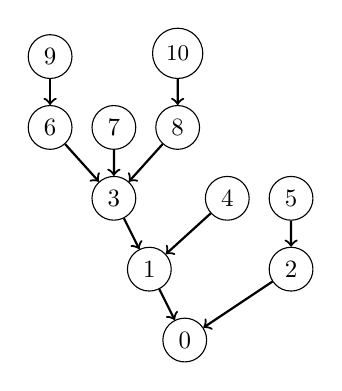
\begin{tikzpicture}[scale=.6, anchor=south]
      \node[circle, scale=0.9, draw] (tid0) at (3,1.5){0};
      \node[circle, scale=0.9, draw] (tid1) at (2.25,3){1};
      \node[circle, scale=0.9, draw] (tid2) at (1.5,4.5){3};
      \node[circle, scale=0.9, draw] (tid7) at (0.15,6){6};
      \node[circle, scale=0.9, draw] (tid9) at (0.15,7.5){9};
      \draw[<-, thick](tid7) -- (tid9);
      \node[circle, scale=0.9, draw] (tid10) at (1.5,6){7};
      \draw[<-, thick](tid2) -- (tid7);
      \draw[<-, thick](tid2) -- (tid10);
      \node[circle, scale=0.9, draw] (tid3) at (3.9,4.5){4};
      \node[circle, scale=0.9, draw] (tid5) at (2.85,6){8};
      \node[circle, scale=0.9, draw] (tid6) at (2.85,7.5){\small 10};
      \draw[<-, thick](tid5) -- (tid6);
      \draw[<-, thick](tid2) -- (tid5);
      \draw[<-, thick](tid1) -- (tid2);
      \draw[<-, thick](tid1) -- (tid3);
      \node[circle, scale=0.9, draw] (tid4) at (5.25,3){2};
      \node[circle, scale=0.9, draw] (tid8) at (5.25,4.5){5};
      \draw[<-, thick](tid4) -- (tid8);
      \draw[<-, thick](tid0) -- (tid1);
      \draw[<-, thick](tid0) -- (tid4);
    \end{tikzpicture}
    \caption{Labelled version with vertex labels and edges drawn as arrows.}
    \label{fig:intree-example-task-names-directed-edges}
  \end{subfigure}
  \quad
  \begin{subfigure}{.45\textwidth}
    \centering{}
    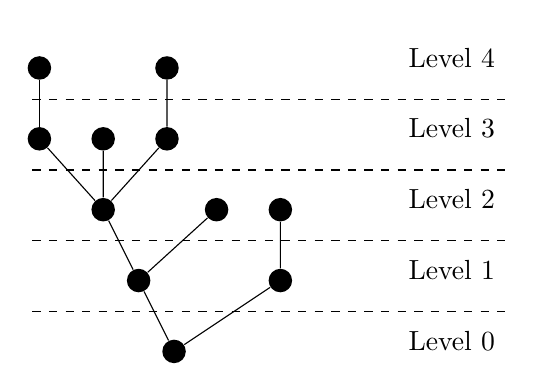
\begin{tikzpicture}[scale=.6, anchor=south]
      \node[circle, scale=0.9, fill] (tid0) at (3,1.5){};
      \node[circle, scale=0.9, fill] (tid1) at (2.25,3){};
      \node[circle, scale=0.9, fill] (tid2) at (1.5,4.5){};
      \node[circle, scale=0.9, fill] (tid7) at (0.15,6){};
      \node[circle, scale=0.9, fill] (tid9) at (0.15,7.5){};
      \draw[](tid7) -- (tid9);
      \node[circle, scale=0.9, fill] (tid10) at (1.5,6){};
      \draw[](tid2) -- (tid7);
      \draw[](tid2) -- (tid10);
      \node[circle, scale=0.9, fill] (tid3) at (3.9,4.5){};
      \node[circle, scale=0.9, fill] (tid5) at (2.85,6){};
      \node[circle, scale=0.9, fill] (tid6) at (2.85,7.5){};
      \draw[](tid5) -- (tid6);
      \draw[](tid2) -- (tid5);
      \draw[](tid1) -- (tid2);
      \draw[](tid1) -- (tid3);
      \node[circle, scale=0.9, fill] (tid4) at (5.25,3){};
      \node[circle, scale=0.9, fill] (tid8) at (5.25,4.5){};
      \draw[](tid4) -- (tid8);
      \draw[](tid0) -- (tid1);
      \draw[](tid0) -- (tid4);
      % level separators
      \draw[dashed] (0, 2.6) -- +(10, 0) node[below left, yshift=-.125cm]{Level 0};
      \draw[dashed] (0, 4.1) -- +(10, 0) node[below left, yshift=-.125cm]{Level 1};
      \draw[dashed] (0, 5.6) -- +(10, 0) node[below left, yshift=-.125cm]{Level 2};
      \draw[dashed] (0, 7.1) -- +(10, 0) node[below left, yshift=-.125cm]{Level 3};
      \draw[      ] (0, 8.6)    +(10, 0) node[below left, yshift=-.125cm]{Level 4};
    \end{tikzpicture}
    \caption{Unlabelled without arrows, edges are implicitly towards the root.}
    \label{fig:intree-example-structure-version}
  \end{subfigure}
  \caption{Graphical representation of an intree with 5 levels (numbered 0 to 4). All edges are implicitly directed towards the root, which is drawn at the bottom of the tree. Most of the time, the \emph{structure} of the tree is enough, so we will omit vertex names most of the time.}
  \label{fig:intrees-introductory-explanation}
\end{figure}

\begin{definition}[Level]
  Let $I$ be an intree. Let $v$ be a vertex within $I$. We define $level(v)$ be number of edges along the (unique) path from $v$ to the root.
\end{definition}

The concept of levels is illustrated in figure \ref{fig:intrees-introductory-explanation}.

\todo{Anzahl der rooted trees angeben.}
\todo{Forest!}

\section{Schedules}
\label{sec:introduction-schedules}

We have seen in section \ref{sec:foundations-graph-theory} how we can interpret an intree as a collection of tasks that have certain dependencies among each other (each task is directly required for \emph{at most} one other task). 

\paragraph{Random task times} \todo{Sollte das wo anders rein?}

We now assume that we do not know the processing time for a certain task in advance. We instead assume that we can model the task time for each task within the intree by an exponentially distributed random variable as defined in section \ref{sec:exponential-distribution}. We furthermore assume that all tasks are exponentially distributed with the \emph{same} parameter $\lambda$. Note that we can assume -- according to theorem \ref{thm:expoenential-distr-scalability} -- $\lambda=1$.\todo{More explanation}

We now assume that we have a certain amount $p$ of identical processors, and we want to process all tasks in an intree (of course in a valid order) such that the overall processing time is minimized. I.e. we want to mimimize the point of time, where the root's processing is done.

We assume that one single task can be processed by one processor exclusively, i.e. it is not possible to save time by ``splitting'' one single task over several processors. That, moreover, means that there might be idle processors if we have more ready tasks than processors. \todo{Define ready tasks!}

We furthermore work with non-preemtive scheduling, i.e. once a task is processor is assigned a task, this task has to be processed \emph{completely} before the processor can be used for anything else.

\section{Computing the expected run time of a schedule}
\label{sec:introduction-compute-expected-time-schedule}

\todo{Snapshot definieren!}

If we want to process a whole intree of tasks, we have to do so step by step, of course. That is, we assign some tasks to processors, wait until the first task finishes, assign a new task (if available) to the now idle processor, and continue with the subtree obtained by removing the finished task. That is, in each point of time, we know the current intree containing all tasks not yet finished and all tasks currently being processed. We therefore introduce the notation of \emph{snapshots}.

\begin{definition}[Snapshot]
  Let $I$ be an intree and let $S$ be a schedule.
  A \emph{snapshot} of $S$ a 2-tuple containing
  \begin{itemize}
  \item The current subtree $I'\subseteq I$ describing which tasks are not finished.
  \item A set $X$ holding the tasks that are currently being processed.
  \end{itemize}
\end{definition}

While the above definition is well suited for theoretical considerations, we -- most of the time -- are satisfied with a concise graphical representation, that will look as shown in figure \ref{fig:intro-snapshot-graphical-representation}.

\begin{figure}[t]
  \centering
  \begin{tikzpicture}[scale=.2, anchor=south]
    \node[circle, scale=0.75, fill] (tid0) at (3,1.5){};
    \node[circle, scale=0.75, fill] (tid1) at (1.5,3){};
    \node[circle, scale=0.75, fill] (tid3) at (0.75,4.5){};
    \node[circle, scale=0.75, fill] (tid4) at (2.25,4.5){};
    \node[circle, scale=0.75, fill, task_scheduled] (tid7) at (2.25,6){};
    \draw[](tid4) -- (tid7);
    \draw[](tid1) -- (tid3);
    \draw[](tid1) -- (tid4);
    \node[circle, scale=0.75, fill] (tid2) at (3.75,3){};
    \node[circle, scale=0.75, fill] (tid5) at (5.25,3){};
    \node[circle, scale=0.75, fill, task_scheduled] (tid6) at (5.25,4.5){};
    \draw[](tid5) -- (tid6);
    \draw[](tid0) -- (tid1);
    \draw[](tid0) -- (tid2);
    \draw[](tid0) -- (tid5);
    % arrows for scheduled tasks
    \draw(tid7) +(1,0)[<-, thick] ..controls+(4,0) and +(0,1).. (15,3);
    \draw(tid6) +(1,0)[<-, thick] ..controls+(2,0) and +(0,1).. (15,3) 
    node[below]{scheduled tasks};
    % brace for whole intree
    \draw[decorate, decoration=brace](-1,1) --node[left, xshift=-.1cm]{current intree} +(0,7);
  \end{tikzpicture}
  \caption{A snapshot is determined by its intree and a collection of currently scheduled tasks.}
  \label{fig:intro-snapshot-graphical-representation}
\end{figure}

If we are speaking of a schedule, we can think of it as a directed acyclic graph, where each vertex represents one single snapshot. The edges between the snapshots then represent transitions that indicate that a certain task has finished. We can naturally assign the edges weights that represent the corresponding probability that a task has finished.\todo{Dag definieren? Oder Verweis auf irgendwen?}

Computing the expected run time for a given schedule (more precisely for the whole processing of an intree according to a certain schedule) can be easily acchieved via a recursive formula that can be explained as follows:

\begin{itemize}
\item If the current intree $I$ consists of exactly one task (the root), then we simply have to process this single task. Since one task has expected run time $\frac{1}{\lambda}=1$ (remember: we assumed w.l.o.g $\lambda=1$), we know that the expected run time for $I$ is 1.
\item If the current intree consists of more than 1 task, there may be up to $p$ tasks scheduled. Let us assume that there are $r\leq p$ tasks scheduled and denote the set of these tasks by $X=\{x_1,x_2,\dots,x_r\}$. According to theorem (\ref{eq:probability-that-cont-random-variable-is-smallest-out-of-iid-is-one-over-n}), the probability that task $x_i$ ($i\in\left\{ 1,2,\dots,r \right\}$) is the \emph{first} task to finish is $\frac{1}{r}$. The expected run time for $x_i$ is $\frac{1}{n}$ (by theorems \ref{thm:minimum-of-exponential-distribution-is-exponential} and \ref{thm:exponential-distribution-expectancy}).

  If task $x_i$ finishes, the remaining intree is $I\setminus\left\{ x_i \right\}$ \todo{Define setminus for trees!}, with -- due to non-preemtive scheduling -- at least tasks $\left\{ x_1,x_2,\dots,x_r \right\} \setminus \left\{ x_i \right\}$ scheduled. By $X_i$ we denote the set of tasks that are scheduled in the next step ($\left\{ x_1,x_2,\dots,x_r \right\} \setminus \left\{ x_i \right\} \subseteq X'$). The expected run time for $I\setminus\left\{ x_i \right\}$ can then be computed recursively.

  This means: If $x_i$ is the first task to finish, the expected run time is given by
  \begin{equation*}
    \frac{1}{r} + T_{X_i}(I\setminus\left\{ x_i \right\}),
  \end{equation*}
  where $T_{X_i}(I\setminus\left\{ x_i \right\})$ denotes the expected run time for the intree $I\setminus\left\{ x_i \right\}$ if the tasks within $X_i$ are scheduled.

  Since each one of the tasks $x_1,x_2,\dots,x_r$ can be the first task to finish, we can compute the overal run time by \todo{Bedingte Wahrscheinlichkeitssumme einführen}
  \begin{eqnarray}
    \nonumber
    T_X(I) 
    &=& 
    \sum_{i=1}^r \frac{1}{r} \cdot \left( \frac{1}{r} + T_{X_i}\left( I\setminus\left\{ x_i \right\} \right) \right) = \\
    \label{eqn:intro-recursive-formula-for-run-time}
    &=&     
    \frac{1}{r} + \frac{1}{r} \cdot \sum_{i=1}^r T_{X_i}\left( I\setminus\left\{ x_i \right\} \right).
  \end{eqnarray}
\end{itemize}

\emph{Remark:} The fact that we can compute the expected run time recursively follows from the fact that exponentially distributed random variables are memoryless (see theorem \ref{thm:exponential-memoryless}): If one task finishes, the remaining tree can be considered \emph{as if} we just started the scheduled tasks. Thus, we are in the same situation as before, except that we have one task less.\todo{Verbessern.}

As an example, consider the tree in figure \ref{fig:intro-computing-expected-runtime}. The topmost snapshots are the ones whose expected run times we are interested in. The run times of the snapshots in the second line are already computed. Using these, we can compute the overal expected run time.

\begin{figure}[tt]
  \centering
  \begin{subfigure}{.45\textwidth}
    \renewcommand{\leveltopI}{-15cm + \leveltop}
    \renewcommand{\leveltopII}{-15cm + \leveltopI}
    \renewcommand{\leveltopIII}{-15cm + \leveltopII}
    \centering
    \begin{tikzpicture}[scale=.2, anchor=south]
      \begin{scope}[yshift=\leveltopI cm]
        \matrix (line1)[column sep=.5cm] {
          \node[draw=black, rectangle split,  rectangle split parts=2] (sn0x834df78){
            \begin{tikzpicture}[scale=.2]
              \node[circle, scale=0.75, fill] (tid0) at (3,1.5){};
              \node[circle, scale=0.75, fill] (tid1) at (2.25,3){};
              \node[circle, scale=0.75, fill, task_scheduled] (tid2) at (0.75,4.5){};
              \node[circle, scale=0.75, fill] (tid4) at (3,4.5){};
              \node[circle, scale=0.75, fill] (tid5) at (2.25,6){};
              \node[circle, scale=0.75, fill] (tid7) at (2.25,7.5){};
              \node[circle, scale=0.75, fill, task_scheduled] (tid8) at (2.25,9){};
              \draw[](tid7) -- (tid8);
              \draw[](tid5) -- (tid7);
              \node[circle, scale=0.75, fill, task_scheduled] (tid6) at (3.75,6){};
              \draw[](tid4) -- (tid5);
              \draw[](tid4) -- (tid6);
              \draw[](tid1) -- (tid2);
              \draw[](tid1) -- (tid4);
              \node[circle, scale=0.75, fill] (tid3) at (5.25,3){};
              \draw[](tid0) -- (tid1);
              \draw[](tid0) -- (tid3);
            \end{tikzpicture}
            \nodepart{two}
            \footnotesize{6.21811}
          };
          & 
          \\
        };
      \end{scope}
      \begin{scope}[yshift=\leveltopII cm]
        \matrix (line2)[column sep=.5cm] {
          \node[draw=black, rectangle split,  rectangle split parts=2] (sn0x834f4d0){
            \begin{tikzpicture}[scale=.2]
              \node[circle, scale=0.75, fill] (tid0) at (3,1.5){};
              \node[circle, scale=0.75, fill] (tid1) at (2.25,3){};
              \node[circle, scale=0.75, fill, task_scheduled] (tid2) at (0.75,4.5){};
              \node[circle, scale=0.75, fill] (tid4) at (3,4.5){};
              \node[circle, scale=0.75, fill] (tid5) at (2.25,6){};
              \node[circle, scale=0.75, fill, task_scheduled] (tid7) at (2.25,7.5){};
              \draw[](tid5) -- (tid7);
              \node[circle, scale=0.75, fill, task_scheduled] (tid6) at (3.75,6){};
              \draw[](tid4) -- (tid5);
              \draw[](tid4) -- (tid6);
              \draw[](tid1) -- (tid2);
              \draw[](tid1) -- (tid4);
              \node[circle, scale=0.75, fill] (tid3) at (5.25,3){};
              \draw[](tid0) -- (tid1);
              \draw[](tid0) -- (tid3);
            \end{tikzpicture}
            \nodepart{two}
            \footnotesize{5.41204}
          };
          & 
          \node[draw=black, rectangle split,  rectangle split parts=2] (sn0x834ec08){
            \begin{tikzpicture}[scale=.2]
              \node[circle, scale=0.75, fill] (tid0) at (2.25,1.5){};
              \node[circle, scale=0.75, fill] (tid1) at (1.5,3){};
              \node[circle, scale=0.75, fill, task_scheduled] (tid2) at (0.75,4.5){};
              \node[circle, scale=0.75, fill] (tid4) at (2.25,4.5){};
              \node[circle, scale=0.75, fill] (tid5) at (2.25,6){};
              \node[circle, scale=0.75, fill] (tid7) at (2.25,7.5){};
              \node[circle, scale=0.75, fill, task_scheduled] (tid8) at (2.25,9){};
              \draw[](tid7) -- (tid8);
              \draw[](tid5) -- (tid7);
              \draw[](tid4) -- (tid5);
              \draw[](tid1) -- (tid2);
              \draw[](tid1) -- (tid4);
              \node[circle, scale=0.75, fill, task_scheduled] (tid3) at (3.75,3){};
              \draw[](tid0) -- (tid1);
              \draw[](tid0) -- (tid3);
            \end{tikzpicture}
            \nodepart{two}
            \footnotesize{6.09066}
          };
          & 
          \node[draw=black, rectangle split,  rectangle split parts=2] (sn0x834f908){
            \begin{tikzpicture}[scale=.2]
              \node[circle, scale=0.75, fill] (tid0) at (2.25,1.5){};
              \node[circle, scale=0.75, fill] (tid1) at (1.5,3){};
              \node[circle, scale=0.75, fill] (tid4) at (1.5,4.5){};
              \node[circle, scale=0.75, fill] (tid5) at (0.75,6){};
              \node[circle, scale=0.75, fill] (tid7) at (0.75,7.5){};
              \node[circle, scale=0.75, fill, task_scheduled] (tid8) at (0.75,9){};
              \draw[](tid7) -- (tid8);
              \draw[](tid5) -- (tid7);
              \node[circle, scale=0.75, fill, task_scheduled] (tid6) at (2.25,6){};
              \draw[](tid4) -- (tid5);
              \draw[](tid4) -- (tid6);
              \draw[](tid1) -- (tid4);
              \node[circle, scale=0.75, fill, task_scheduled] (tid3) at (3.75,3){};
              \draw[](tid0) -- (tid1);
              \draw[](tid0) -- (tid3);
            \end{tikzpicture}
            \nodepart{two}
            \footnotesize{6.15162}
          };
          & 
          \\
        };
      \end{scope}
      \draw (sn0x834df78.south) -- (sn0x834f4d0.north);
      \draw (sn0x834df78.south) -- (sn0x834ec08.north);
      \draw (sn0x834df78.south) -- (sn0x834f908.north);
    \end{tikzpicture}
    \caption{Three processors. 
      Transition probabilities are $\frac{1}{3}$ each.
      Then, we can compute $
      \frac{1}{3}+\frac{1}{3}\cdot
      \left( 
        5.41204 + 6.09066 + 6.15162
      \right)
      = 6.21811$.
    }
  \end{subfigure}
  \quad
  \begin{subfigure}{.45\textwidth}
    \centering
    \renewcommand{\leveltopI}{-15cm + \leveltop}
    \renewcommand{\leveltopII}{-15cm + \leveltopI}
    \renewcommand{\leveltopIII}{-15cm + \leveltopII}
    \renewcommand{\leveltopIIII}{-15cm + \leveltopIII}
    \renewcommand{\leveltopIIIII}{-15cm + \leveltopIIII}
    \renewcommand{\leveltopIIIIII}{-15cm + \leveltopIIIII}
    \renewcommand{\leveltopIIIIIII}{-15cm + \leveltopIIIIII}
    \renewcommand{\leveltopIIIIIIII}{-15cm + \leveltopIIIIIII}
    \renewcommand{\leveltopIIIIIIIII}{-15cm + \leveltopIIIIIIII}
    \begin{tikzpicture}[scale=.2, anchor=south]
      \begin{scope}[yshift=\leveltopI cm]
        \matrix (line1)[column sep=.5cm] {
          \node[draw=black, rectangle split,  rectangle split parts=2] (sn0x9500f78){
            \begin{tikzpicture}[scale=.2]
              \node[circle, scale=0.75, fill] (tid0) at (3,1.5){};
              \node[circle, scale=0.75, fill] (tid1) at (2.25,3){};
              \node[circle, scale=0.75, fill, task_scheduled] (tid2) at (0.75,4.5){};
              \node[circle, scale=0.75, fill] (tid4) at (3,4.5){};
              \node[circle, scale=0.75, fill] (tid5) at (2.25,6){};
              \node[circle, scale=0.75, fill] (tid7) at (2.25,7.5){};
              \node[circle, scale=0.75, fill, task_scheduled] (tid8) at (2.25,9){};
              \draw[](tid7) -- (tid8);
              \draw[](tid5) -- (tid7);
              \node[circle, scale=0.75, fill, task_scheduled] (tid6) at (3.75,6){};
              \draw[](tid4) -- (tid5);
              \draw[](tid4) -- (tid6);
              \draw[](tid1) -- (tid2);
              \draw[](tid1) -- (tid4);
              \node[circle, scale=0.75, fill, task_scheduled] (tid3) at (5.25,3){};
              \draw[](tid0) -- (tid1);
              \draw[](tid0) -- (tid3);
            \end{tikzpicture}
            \nodepart{two}
            \footnotesize{6.20264}
          };
          & 
          \\
        };
      \end{scope}
      \begin{scope}[yshift=\leveltopII cm]
        \matrix (line2)[column sep=.5cm] {
          \node[draw=black, rectangle split,  rectangle split parts=2] (sn0x9502500){
            \begin{tikzpicture}[scale=.2]
              \node[circle, scale=0.75, fill] (tid0) at (3,1.5){};
              \node[circle, scale=0.75, fill] (tid1) at (2.25,3){};
              \node[circle, scale=0.75, fill, task_scheduled] (tid2) at (0.75,4.5){};
              \node[circle, scale=0.75, fill] (tid4) at (3,4.5){};
              \node[circle, scale=0.75, fill] (tid5) at (2.25,6){};
              \node[circle, scale=0.75, fill, task_scheduled] (tid7) at (2.25,7.5){};
              \draw[](tid5) -- (tid7);
              \node[circle, scale=0.75, fill, task_scheduled] (tid6) at (3.75,6){};
              \draw[](tid4) -- (tid5);
              \draw[](tid4) -- (tid6);
              \draw[](tid1) -- (tid2);
              \draw[](tid1) -- (tid4);
              \node[circle, scale=0.75, fill, task_scheduled] (tid3) at (5.25,3){};
              \draw[](tid0) -- (tid1);
              \draw[](tid0) -- (tid3);
            \end{tikzpicture}
            \nodepart{two}
            \footnotesize{5.39005}
          };
          & 
          \node[draw=black, rectangle split,  rectangle split parts=2] (sn0x9501c08){
            \begin{tikzpicture}[scale=.2]
              \node[circle, scale=0.75, fill] (tid0) at (2.25,1.5){};
              \node[circle, scale=0.75, fill] (tid1) at (1.5,3){};
              \node[circle, scale=0.75, fill, task_scheduled] (tid2) at (0.75,4.5){};
              \node[circle, scale=0.75, fill] (tid4) at (2.25,4.5){};
              \node[circle, scale=0.75, fill] (tid5) at (2.25,6){};
              \node[circle, scale=0.75, fill] (tid7) at (2.25,7.5){};
              \node[circle, scale=0.75, fill, task_scheduled] (tid8) at (2.25,9){};
              \draw[](tid7) -- (tid8);
              \draw[](tid5) -- (tid7);
              \draw[](tid4) -- (tid5);
              \draw[](tid1) -- (tid2);
              \draw[](tid1) -- (tid4);
              \node[circle, scale=0.75, fill, task_scheduled] (tid3) at (3.75,3){};
              \draw[](tid0) -- (tid1);
              \draw[](tid0) -- (tid3);
            \end{tikzpicture}
            \nodepart{two}
            \footnotesize{6.09066}
          };
          & 
          \node[draw=black, rectangle split,  rectangle split parts=2] (sn0x95028b8){
            \begin{tikzpicture}[scale=.2]
              \node[circle, scale=0.75, fill] (tid0) at (2.25,1.5){};
              \node[circle, scale=0.75, fill] (tid1) at (1.5,3){};
              \node[circle, scale=0.75, fill] (tid4) at (1.5,4.5){};
              \node[circle, scale=0.75, fill] (tid5) at (0.75,6){};
              \node[circle, scale=0.75, fill] (tid7) at (0.75,7.5){};
              \node[circle, scale=0.75, fill, task_scheduled] (tid8) at (0.75,9){};
              \draw[](tid7) -- (tid8);
              \draw[](tid5) -- (tid7);
              \node[circle, scale=0.75, fill, task_scheduled] (tid6) at (2.25,6){};
              \draw[](tid4) -- (tid5);
              \draw[](tid4) -- (tid6);
              \draw[](tid1) -- (tid4);
              \node[circle, scale=0.75, fill, task_scheduled] (tid3) at (3.75,3){};
              \draw[](tid0) -- (tid1);
              \draw[](tid0) -- (tid3);
            \end{tikzpicture}
            \nodepart{two}
            \footnotesize{6.15162}
          };
          & 
          \node[draw=black, rectangle split,  rectangle split parts=2] (sn0x9502a20){
            \begin{tikzpicture}[scale=.2]
              \node[circle, scale=0.75, fill] (tid0) at (2.25,1.5){};
              \node[circle, scale=0.75, fill] (tid1) at (2.25,3){};
              \node[circle, scale=0.75, fill, task_scheduled] (tid2) at (0.75,4.5){};
              \node[circle, scale=0.75, fill] (tid4) at (3,4.5){};
              \node[circle, scale=0.75, fill] (tid5) at (2.25,6){};
              \node[circle, scale=0.75, fill] (tid7) at (2.25,7.5){};
              \node[circle, scale=0.75, fill, task_scheduled] (tid8) at (2.25,9){};
              \draw[](tid7) -- (tid8);
              \draw[](tid5) -- (tid7);
              \node[circle, scale=0.75, fill, task_scheduled] (tid6) at (3.75,6){};
              \draw[](tid4) -- (tid5);
              \draw[](tid4) -- (tid6);
              \draw[](tid1) -- (tid2);
              \draw[](tid1) -- (tid4);
              \draw[](tid0) -- (tid1);
            \end{tikzpicture}
            \nodepart{two}
            \footnotesize{6.17824}
          };
          & 
          \\
        };
      \end{scope}
      \draw (sn0x9500f78.south) -- (sn0x9502500.north);
      \draw (sn0x9500f78.south) -- (sn0x9501c08.north);
      \draw (sn0x9500f78.south) -- (sn0x95028b8.north);
      \draw (sn0x9500f78.south) -- (sn0x9502a20.north);
    \end{tikzpicture}
    \caption{Four processors. Transition probabilities between snapshots are $\frac{1}{4}$ each, so we can compute the overal expected run time by 
      $
      \frac{1}{4} + \frac{1}{4}\cdot 
      \left( 
        5.39005 + 6.09066 + 6.15162 + 6.17824
      \right)
      = 6.20264
      $
    }
  \end{subfigure}
  \caption{Computing the expected run time according to equation (\ref{eqn:intro-recursive-formula-for-run-time}) for three resp. four processors on the same intree. Each box represents a single snapshot.}
  \label{fig:intro-computing-expected-runtime}
\end{figure}

%%% Local Variables:
%%% TeX-master: "../thesis.tex"
%%% End: 